% This file was created with tikzplotlib v0.10.1.
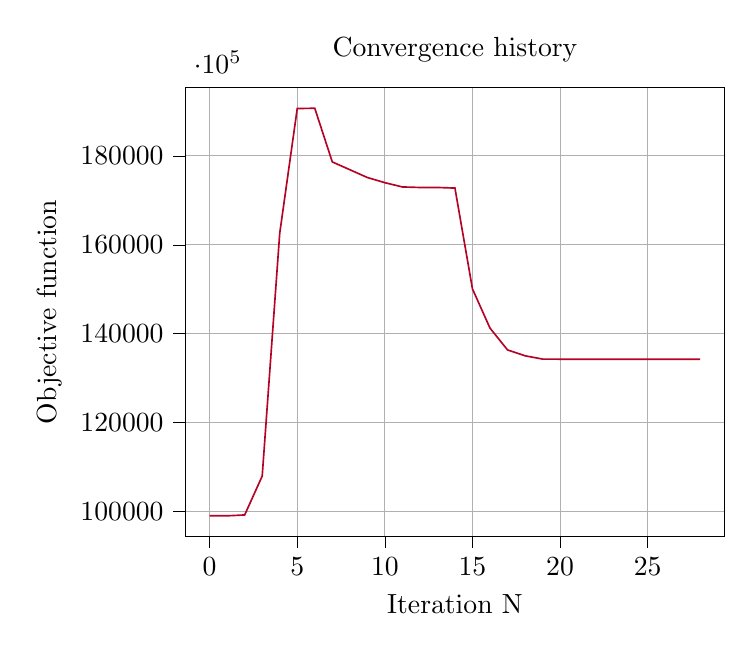
\begin{tikzpicture}

\definecolor{darkgray176}{RGB}{176,176,176}
\definecolor{firebrick180438}{RGB}{180,4,38}

\begin{axis}[
tick align=outside,
tick pos=left,
title={Convergence history},
x grid style={darkgray176},
xlabel={Iteration N},
xmajorgrids,
xmin=-1.4, xmax=29.4,
xtick style={color=black},
xtick={-5,0,5,10,15,20,25,30},
xticklabels={
  \(\displaystyle {\ensuremath{-}5}\),
  \(\displaystyle {0}\),
  \(\displaystyle {5}\),
  \(\displaystyle {10}\),
  \(\displaystyle {15}\),
  \(\displaystyle {20}\),
  \(\displaystyle {25}\),
  \(\displaystyle {30}\)
},
y grid style={darkgray176},
ylabel={Objective function},
ymajorgrids,
ymin=94484.3437438669, ymax=195281.951456394,
ytick style={color=black},
ytick={80000,100000,120000,140000,160000,180000,200000},
yticklabels={
  \(\displaystyle {80000}\),
  \(\displaystyle {100000}\),
  \(\displaystyle {120000}\),
  \(\displaystyle {140000}\),
  \(\displaystyle {160000}\),
  \(\displaystyle {180000}\),
  \(\displaystyle {200000}\)
}
]
\addplot [semithick, firebrick180438]
table {%
0 99066.0531853454
1 99066.0531853454
2 99257.5651575967
3 107997.641783494
4 162574.922660599
5 190636.992194726
6 190700.242014915
7 178633.5322492
8 176881.372477471
9 175130.663571965
10 173963.405200494
11 173008.763165691
12 172886.108892368
13 172886.108892368
14 172756.273550626
15 150086.797850829
16 141278.236051614
17 136369.166142955
18 135045.869080736
19 134305.182289336
20 134281.17508875
21 134279.382090986
22 134279.340537351
23 134279.326357676
24 134279.324484325
25 134279.324422338
26 134279.324421918
27 134279.324421918
28 134279.324421918
};
\end{axis}

\end{tikzpicture}
